\documentclass[aps,prx,reprint,floatfix,superscriptaddress,nofootinbib]{revtex4-2}
\usepackage[T1]{fontenc}
\usepackage[utf8]{inputenc}
\usepackage{amsmath,amssymb,bm,amsthm}
\usepackage{graphicx}
\usepackage{booktabs}
\usepackage[hidelinks]{hyperref}
\hypersetup{pdftitle={Self-Consistent Loss Geometries and the Laws of Learning},pdfauthor={Gerard McCaul},pdfsubject={Full standalone manuscript candidate}}
\newtheorem{proposition}{Proposition}
\newtheorem{theorem}{Theorem}
\begin{document}
\title{Self-Consistent Loss Geometries and the Laws of Learning}
\author{Gerard McCaul}
\date{11 November 2026}
\begin{abstract}
A learner with finite representational resources must decide how to change its model, which changes deserve authority and when additional capacity is worth buying. We develop a finite framework in which the evaluator can itself be part of the regulated state. A shared quadratic register supplies a common cost ledger and an exact boundary between reuse, arbitration and partition purchase. Relative-entropy regularisation gives a normalised selector over available actions, with gains evaluated at the states those actions execute. A separately specified model/evaluator controller converges in reuse mode under stated damping and coupling conditions, without assuming that convergence establishes adaptive value. We derive weighted free-energy contraction and show that OR aggregation of externally frozen independent update opportunities closes exactly in cumulative hazard. A smaller common-intercept representation has a calculable event-probability error, while its threshold response equals conditional event multiplicity. The distinction between marginalisation and constrained closure also leads to a quantum recovery criterion. A matched synthetic policy comparison exposes the difference between consistent action pricing and predictive success, retaining the adverse predictive result. The proposed laws of learning are operational requirements on an embodied model-revision scheme: declare its evaluator, price its executed actions, and test what survives a change of representation.

\end{abstract}
\maketitle
\section{Introduction}
\label{sec:yba-introduction}

Consider one memory register used by two tasks. Each task would set the register to a different value. Moving it towards one target moves it away from the other. The learner can change the register, change the relative authority of the tasks, or buy a second register. These are different operations. No amount of care in taking the gradient of a fixed objective will make the third operation appear if the architecture permits only the first two.

The difficulty becomes sharper when the learner must decide for itself which operation is worth making. Its estimate of future benefit depends on the model it currently has. Its estimate of the cost depends on the memory, controller and action repertoire through which that model is implemented. A proposed revision can alter both. The evaluator is therefore not merely a number attached to the model by an observer. It is a mechanism within the loop, with a state, inputs and an update protocol of its own.

This does not make a supplied loss illegitimate. An engineering problem can specify a target externally and ask an algorithm to optimise it. Our question begins where that description stops: how should we describe a learner that regulates its own model revision, including the allocation of a shared representation? We need to distinguish three things that are easily conflated. A controller may be internally consistent, it may converge, and it may improve an external task. None of these properties alone supplies the other two.

We develop the argument from the register rather than introducing a universal objective. Two quadratic demands let us calculate the cost of shared allocation exactly. An explicit split option then identifies when purchasing capacity is cheaper than continuing to arbitrate. The result is a price boundary, not a claim that a larger model must generalise better. Every option is compared on the same ledger.

The next step is to give the learner actual actions. A model revision must be scored at the state it will reach, not at an ideal fit that the implementation never executes. For a partial least-squares move, the difference can reverse the decision to update. With those actions specified, a finite relative-entropy objective produces a Gibbs selector relative to a declared reference measure. The statistical mechanics is a variational construction, not an assumption that the learner contains a thermostat or samples all its alternatives.

We then put an evaluator on the opening register. Its model coordinate and authority weight adapt together under a simple, explicitly postulated controller. This gives a concrete self-consistent loss geometry: a loss family, a metric, a model step and an evaluator step whose joint stationary states can be studied. The construction admits a rigorous convergence region. Its usefulness is precisely that we can say what converges and why, without identifying a stable internal agreement with successful regulation of the world.

A finite learner also needs descriptions smaller than its complete history. We therefore ask what remains when update opportunities are aggregated. Weighted free-energy contraction gives an exact answer for finite hidden alternatives. For the event that at least one of several independent opportunities produces an update, the retained quantity is cumulative hazard. Keeping only a summed margin and one common threshold is a further approximation. Its error can be measured, and its response to repricing has a simple meaning: the expected number of fine events conditional on any event occurring.

These calculations give the phrase \emph{laws of learning} its intended scope. We propose three requirements for this class of embodied model-revision schemes. \emph{Endogenous evaluation} requires an explicit description of the evaluator when it is part of the learner. \emph{Embodied price} requires a common ledger for the actions actually performed. \emph{Representation covariance} requires a declared receiving representation and a test of which predictions or transitions it preserves. The requirements organise a model class. The finite theorems follow from the premises stated beside them, not from a claim that every biological learner obeys our controller.

The paper is self-contained. Section~\ref{sec:yba-setup} derives the register purchase. Section~\ref{sec:self-consistent-loss-geometry} constructs the action selector and coupled regulator. Section~\ref{sec:partition-covariance-reuse} moves the construction inside a larger controller. Section~\ref{sec:numerical-demonstrations} examines a synthetic tracking problem and retains the finding that consistent action pricing does not deliver a predictive victory. Section~\ref{sec:yba-examples} develops exact contraction, the OR example and dynamical receiving-map tests. We then identify the primary methods used and develop the consequences for further modelling. The appendices provide proofs, the complete finite protocol and the quantum extension.

\section{When a shared register should split}
\label{sec:yba-setup}

The opening problem needs a cost ledger before it needs an algorithm. Let \(q\in\mathbb R^2\) be a shared register, and let \(a,b\in\mathbb R^2\) be unit target vectors separated by angle \(\theta\in[0,\pi]\). Write
\begin{align}
 d^2&=\|a-b\|^2=2(1-\cos\theta),\nonumber\\
 \ell_1(q)&=\frac12\|q-a\|^2,\qquad
 \ell_2(q)=\frac12\|q-b\|^2 .
 \label{eq:num-toy-evaluator-losses}
\end{align}
The tasks supply distinct demands on one physical state. An authority weight \(\alpha\in[0,1]\) assigns task 1 a share \(\alpha\) and task 2 a share \(1-\alpha\). The weight is not an additional register in which both targets can be stored independently.

We choose the dimensionless static ledger
\begin{align}
 J(q,\alpha)={}&\alpha\ell_1(q)+(1-\alpha)\ell_2(q)
       +\gamma\alpha(1-\alpha)d^2 \nonumber\\
 &+\eta\big[(\alpha-\tfrac12)^2+
                  (1-\alpha-\tfrac12)^2\big],
 \qquad \gamma,\eta\geq0 .
 \label{eq:num-toy-conflict}
\end{align}
The first terms score the tasks. The term proportional to \(\gamma\) charges simultaneous incompatible use. The term proportional to \(\eta\) makes withdrawing authority from either task costly. These are declared modelling choices. Geometry alone does not force this particular conflict penalty, and a different physical ledger can produce a different purchase boundary.

For fixed \(\alpha\), differentiation with respect to the register gives
\begin{equation}
 q^*(\alpha)=\alpha a+(1-\alpha)b .
 \label{eq:num-toy-agent-b-optimum}
\end{equation}
Substituting this state eliminates the routine register motion. The weighted task residual becomes \(\alpha(1-\alpha)d^2/2\). If
\(A=d^2(1/2+\gamma)\), the entire remaining decision is
\begin{equation}
 J_{\mathrm{red}}(\alpha)
 =\frac A4+(2\eta-A)(\alpha-\tfrac12)^2 .
 \label{eq:num-toy-reduced-loss}
\end{equation}
A change of representation has already done useful work. Instead of following two components of \(q\) while changing an authority weight, we can decide the optimal allocation from the sign of one coefficient.

When \(A<2\eta\), balance is the unique optimum. When \(A>2\eta\), the two endpoints are optimal and one task receives all authority. At \(A=2\eta\), every allocation ties. Hence the best shared-register cost is
\begin{equation}
 J_{\mathrm{shared}}^*=\min\!\left(\frac A4,\frac\eta2\right).
 \label{eq:shared-minimum}
\end{equation}
Endpoint allocation does not satisfy both tasks. It pays the fairness price in order to stop paying the increasing shared residual and conflict cost. The plateau is an allocation decision, not the disappearance of the neglected task.

Now admit a different operation. The learner may purchase separate registers \(q_1,q_2\), set them to \(a,b\), and maintain balanced authority. We assume that this option has zero task residual and zero shared conflict, at a declared total price \(C_{\mathrm{part}}\geq0\). This price includes whatever maintenance or switching expense is being compared over the chosen static horizon. It is not automatically the one-step price of adding memory in a dynamical system. The enabled option has value
\begin{equation}
 J_{\mathrm{enabled}}^*
 =\min\!\left(\frac A4,\frac\eta2,C_{\mathrm{part}}\right).
 \label{eq:num-toy-agent-c-optimum}
\end{equation}
The strict split region is \(C_{\mathrm{part}}<J_{\mathrm{shared}}^*\). Since \(A\leq4(1/2+\gamma)\), such a region exists somewhere on \([0,\pi]\) precisely when
\begin{equation}
 C_{\mathrm{part}}<\min\!\left(\frac\eta2,\frac12+\gamma\right).
 \label{eq:split-region}
\end{equation}

Figure~\ref{fig:num-toy-shared-register} evaluates this ledger at \(\gamma=1\), \(\eta=0.8\) and \(C_{\mathrm{part}}=0.25\). The first crossing occurs at \(\theta\simeq0.84106867\) radians, where \(A/4=0.25\). Shared arbitration itself reaches its endpoint regime only at \(\theta\simeq1.08527820\), where \(A=1.6\). Capacity is worth buying before abandoning one task becomes the preferred shared solution.

\begin{figure*}[t]
\centering
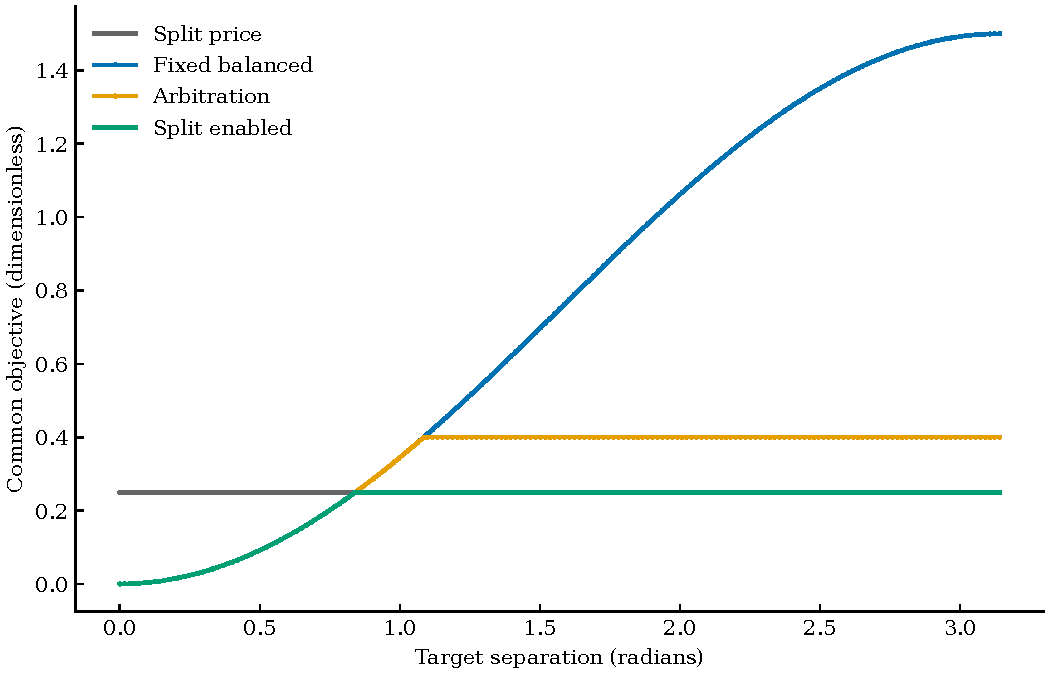
\includegraphics[width=0.82\textwidth]{figures/generated/slg-register-common-ledger-20261111.pdf}
\caption{When splitting the register pays. Static costs on the common ledger in Eq.~\eqref{eq:num-toy-conflict}, evaluated over 181 target separations. Fixed balance costs \(A/4\), optimised arbitration costs \(\min(A/4,0.4)\), and split-enabled allocation costs \(\min(A/4,0.4,0.25)\). All three curves coincide below \(0.8411\) radians, with the green result drawn on top. Above that crossing the green plateau is exactly the grey split-price reference, not a separate lower curve. Arbitration remains equal to fixed balance until \(1.0853\) radians and then caps at \(0.4\). The angle measures target separation. These are calculated static option boundaries, not measured dynamical or biological transitions.}
\label{fig:num-toy-shared-register}
\label{fig:slg-register-common-ledger-20261111}
\end{figure*}

The comparison would be misleading if fixed balance omitted a conflict charge that arbitration had to pay. Its cost here is \(A/4\), not merely the task residual \(d^2/8\). The policy classes are nested, so enabling allocation and then splitting cannot raise their optimised ledger values. The informative calculation is where the extra operation earns its price and which capacity assumption makes that possible.

The geometric interpretation also needs care. At the balanced optimum, the two nonzero task gradients are antiparallel for every \(d>0\). Varying \(\theta\) changes their magnitude, not a gradient angle that rotates continuously from agreement to opposition. In the general allocation optimum,
\(\nabla\ell_1=-(1-\alpha)(a-b)\) and
\(\nabla\ell_2=\alpha(a-b)\).
The register is a clean example of competing demands because those demands and the available operations are visible. To turn the static comparison into learning, we must now specify which state change a controller can actually buy.

\section{A selector for the action actually performed}
\label{sec:self-consistent-loss-geometry}

The static minimum tells an observer which register option is cheapest. A learner needs a decision protocol. Let \(z\in\mathcal Z\) be its complete retained state at one decision. This includes the model \(M\), evaluator parameters \(\lambda\), controller memory and partition label whenever these affect the next transition. Observations available at that decision are \(D\). A finite set \(\mathcal U(z)\) contains executable actions, each with a specified transition \(T_u(z,D)\).

For example, a register-motion action changes \(q\) while holding \(\alpha\) fixed. An arbitration action changes \(\alpha\) while holding \(q\) fixed. A split action changes the partition label and creates the two declared register states. A promotion action changes a persistent model parameter rather than leaving the observation as a transient residual. These transitions may have different effects and horizons. To compare them, freeze one evaluator and one scoring horizon during the decision and define
\begin{equation}
 G_u(z,D)=J_D(z)-J_D(T_u(z,D)),\qquad C_u(z,D)\geq0 .
 \label{eq:actual-gain}
\end{equation}
Here \(J_D\) is the declared score on the candidate state, not necessarily a forecast of future reward. A transient intervention deserves a positive gain only if its effect is represented in \(T_u\) and evaluated by \(J_D\). Staying, \(T_0(z,D)=z\), has \(G_0=0\). An unchanged state can still carry a declared maintenance cost.

\subsection{Finite statistical selection}

Give each available action a positive finite reference mass \(\mu_u\), choose a statistical cost scale \(\tau>0\), and put
\(K_u=C_u-\beta G_u\). The multiplier \(\beta\) converts gain units to cost units. We minimise over probability distributions on the finite action set:
\begin{equation}
 \Phi(P)=\sum_uP_uK_u+
       \tau\sum_uP_u\log\frac{P_u}{\mu_u}.
 \label{eq:selector-objective}
\end{equation}
All logarithms are natural. This is an explicit relative-entropy regularisation premise. The reference masses specify how alternatives are counted before their gains and costs are applied. Changing their ratios changes the selected distribution. A useful special cost arises when declared capacity labels multiply under composition and nondecreasing costs add. Then the cost is proportional to log capacity. Appendix~\ref{app:rank} proves this statement and explains why probability-order ranks need not multiply under independence. The selector itself does not require that special cost.

The unique minimiser is
\begin{equation}
 P_u^*=\frac{\mu_u e^{(\beta G_u-C_u)/\tau}}{Z},
 \qquad Z=\sum_{v\in\mathcal U(z)}\mu_v
                      e^{(\beta G_v-C_v)/\tau}.
 \label{eq:yba-update-ensemble}
\end{equation}
Positivity and finiteness give \(0<Z<\infty\). Substitution writes the objective as
\(\tau D(P\Vert P^*)-\tau\log Z\), proving the result directly. For unnormalised \(\mu\), the expression in Eq.~\eqref{eq:selector-objective} differs from relative entropy to normalised \(\mu\) by a constant. The minimiser is unchanged.

This is the familiar exponential-family construction of maximum-entropy inference \cite{jaynes1957information}, now applied to a declared set of model-revision actions. Its role is to express a variational comparison. One may sample from \(P^*\), or one may use its scores to define a deterministic policy. The latter is what our tracking example does. It does not constitute a test that a physical learner samples a Gibbs ensemble.

For two actions, define \(\sigma(x)=(1+e^{-x})^{-1}\). Their odds give
\begin{align}
 P_1^*&=\sigma\!\left(\log\frac{\mu_1}{\mu_0}+
                                     \frac{\Delta s}{\tau}\right),\nonumber\\
 \Delta s&=\beta(G_1-G_0)-(C_1-C_0).
 \label{eq:two-action}
\end{align}
With equal reference masses, the higher-score policy updates precisely when
\(\beta(G_1-G_0)>C_1-C_0\). We assign equality to staying. For more actions, both the reference convention and a complete tie rule must be specified. A deterministic maximiser is not identical to a finite-temperature distribution.

\subsection{Why a partial action needs its own price}

A scalar tracking problem makes the action identity consequential. Let \(D_t\) be the trailing observations available after observation \(t\), and define the observed-window score
\begin{equation}
 J_t(\vartheta)=\frac1{n_t}\sum_{i\in D_t}
                         (y_i-\vartheta x_i)^2 .
 \label{eq:window-score}
\end{equation}
The current carried model is \(\vartheta\). A rolling ridge target is
\begin{align}
 \vartheta_{\mathrm w}&=
 \frac{\sum_{i\in D_t}x_iy_i}{\sum_{i\in D_t}x_i^2+10^{-6}},
 \qquad \rho=0.22,\nonumber\\
 \vartheta^{(0)}&=\vartheta,\qquad
 \vartheta^{(1)}=\vartheta+\rho(\vartheta_{\mathrm w}-\vartheta).
 \label{eq:actions}
\end{align}
For fewer than eight observations, set \(\vartheta_{\mathrm w}=\vartheta\). The actual-step-priced policy uses
\(G_u=J_t(\vartheta)-J_t(\vartheta^{(u)})\),
\(C_0=0\), \(C_1=c\) and \(\beta=2.5\). If it buys action 1, the next decision starts from \(\vartheta^{(1)}\). Otherwise it carries \(\vartheta\) unchanged. Prediction at observation \(t\) uses the state from before that observation is incorporated.

Write \(v=\vartheta_{\mathrm w}-\vartheta\),
\(A_t=n_t^{-1}\sum x_i^2\) and
\(B_t=n_t^{-1}\sum x_iy_i\). Expanding the quadratic gives
\begin{equation}
 G_1=2\rho v(B_t-A_t\vartheta)-\rho^2v^2A_t .
 \label{eq:partial-gain}
\end{equation}
For an exact unregularised least-squares target with \(A_t>0\),
\begin{equation}
 G_{\mathrm{partial}}=(2\rho-\rho^2)G_{\mathrm{full}}
                     =0.3916G_{\mathrm{full}} .
 \label{eq:partial-factor}
\end{equation}
The ridge target requires Eq.~\eqref{eq:partial-gain} or direct evaluation, not an exact substitution of this least-squares simplification.

Take eight observations \(x_i=1,y_i=0.8\), starting at \(\vartheta=1\). The executed candidate is approximately \(0.955999978\), with gain \(0.0156640069\). Its price-adjusted gain at \(\beta=2.5\) is \(0.0391600172\). At \(c=0.06\) the actual-step policy stays, whereas crediting it with the full-fit improvement, approximately \(0.04\), would authorise a move. At \(c=0.02\) it updates. A subsequent nine-observation call starting from that updated state yields approximately \(0.921679963\). The intervention changes the state on which the next price is calculated. Scoring, executing and carrying are one protocol.

These gains measure fit to observations already available. They are not held-out prediction gains and do not measure future viability. That distinction will matter in Section~\ref{sec:numerical-demonstrations}, where the policy is evaluated on predictions rather than on the score it uses to authorise itself.

\subsection{Putting the evaluator on the register}

The selector requires gains, costs and authority weights to be supplied at each decision. To examine an adapting evaluator separately, return to the opening register with \(d>0\). Let
\(e=(a-b)/d\), \(\bar q=(a+b)/2\), and restrict the reused register to the segment
\begin{align}
 q&=\bar q+\frac d2 m e,\qquad m\in[-1,1],\nonumber\\
 \alpha&=\frac{1+\lambda}{2},\qquad\lambda\in[-1,1].
 \label{eq:register-coordinate}
\end{align}
The task losses become
\(\ell_1=d^2(m-1)^2/8\) and
\(\ell_2=d^2(m+1)^2/8\).
Holding the evaluator coordinate \(\lambda\) fixed,
\begin{equation}
 \partial_m[\alpha\ell_1+(1-\alpha)\ell_2]
                  =\frac{d^2}{4}(m-\lambda).
 \label{eq:register-gradient}
\end{equation}
The conflict and fairness terms depend on \(\alpha\), not on \(m\), so they do not change this partial gradient. For model gradients we use the metric induced by the register coordinate, \(g_{mm}=d^2/4\). The resulting gradient is \(\operatorname{grad}_m J=m-\lambda\), so a step with gain \(a_m\) gives the first component of the following controller. This model metric is distinct from the joint-state norm used below to prove contraction.

We introduce the evaluator step as an \emph{author-chosen model law}:
\begin{align}
 m^+&=(1-a_m)m+a_m\lambda,\nonumber\\
 \lambda^+&=(1-a_\lambda)\lambda+
                      a_\lambda\tanh(km+h).
 \label{eq:regulator}
\end{align}
Both right-hand sides use the old state. We apply this simultaneous map at every reuse-mode step, rather than choosing its components with the action selector. Its model and evaluator domains are \([-1,1]\). The finite parent drive \(h\) is frozen during the convergence analysis. The damping parameters satisfy \(0<a_m,a_\lambda\leq1\), and \(0\leq k<1\). No switching protocol connects this map to the static split comparison.

The square is invariant, because each new coordinate is a convex combination of values in its interval. For any \(k<\nu<1\), use
\(\|(\delta m,\delta\lambda)\|_\nu
 =\max(|\delta m|,|\delta\lambda|/\nu)\).
The Lipschitz constant of the joint map is bounded by
\begin{equation}
 r=\max\!\left(1-a_m+a_m\nu,\,
             1-a_\lambda+a_\lambda k/\nu\right)<1 .
 \label{eq:contraction-factor}
\end{equation}
It follows that there is one fixed point in the square and every initial state converges to it geometrically. The fixed point satisfies
\(m^*=\lambda^*=\tanh(km^*+h)\).
The proof is in Appendix~\ref{app:controller}.

We call the loss family together with this state space, metric and update protocol a \emph{self-consistent loss geometry}. Its stationary evaluator acts on the stationary model, and the stationary model supplies the evaluator's input. This is more informative than an unqualified equation saying that model and loss determine each other. The maps have domains, an update order and a contraction condition.

The controller is not obtained by globally minimising the static reduced allocation objective. In particular, its evaluator postulate need not select the optimal \(\alpha\) of Eq.~\eqref{eq:num-toy-reduced-loss}. Its convergence theorem concerns the declared reuse mode with frozen \(h\). Switching between reuse and split modes, adapting the parent drive or adding controller memory changes the joint map and requires a corresponding analysis.

There is a further distinction at the level of derivatives. The model step holds \(\lambda\) fixed and uses \(\partial_m J(m,\lambda)\). If we instead substitute a state-dependent evaluator \(\lambda=B(m)\) and differentiate \(J(m,B(m))\), the derivative contains the additional term
\(B'(m)\partial_\lambda J\).
These are different update protocols. Treating one as the other quietly changes the model.

Finally, stationarity does not establish alignment with an external improvement field. Let \(g_{\mathrm{ext}}\) be a specified projected, undamped field in the same register-induced model metric. We compare fields, not one-step displacements, using
\begin{equation}
 D_{\mathrm{align}}(m,\lambda)
       =\|-\operatorname{grad}_m J(m,\lambda)-g_{\mathrm{ext}}(m)\|.
 \label{eq:alignment-defect}
\end{equation}
The fixed-point residual instead measures
\(\|(m,\lambda)-T(m,\lambda)\|\).
A zero residual says that the declared controller has settled. A small alignment defect says that its undamped model field is close to the specified target field. The actual model displacement includes the gain \(a_m\). A general target field need not even admit a scalar potential. We therefore keep existence, attraction and alignment as separate questions. The tracking comparison below supplies an especially direct reason to do so.

\section{An evaluator inside a larger controller}
\label{sec:partition-covariance-reuse}

The register/controller pair is already an embedded system. The register receives authority from \(\lambda\), while the evaluator receives a parent drive \(h\). Moving the model/world boundary inside a learner should therefore begin by naming these exchanges, not by attaching a subsystem index to the global equations.

Let the full system state be \(Z\), let \(s=\pi_S(Z)\) be the retained local state of a subsystem \(S\), and let \(b_t\) denote its observed boundary variables. The parent state is \(p_t\). We specify a local action set \(\mathcal U_S(s_t,b_t)\), a transition
\(s_{t+1}=T^S_u(s_t,b_t)\), and a parent signal
\(\widehat{\Delta V}_{S\leftarrow P}(u)\).
The last quantity is the parent's communicated estimate of the consequence of a local action over a declared horizon. It can be a value estimate or an error-derived signal, but it must be converted to the cost units used by the local selector.

With reference masses \(\mu^S_u>0\), local costs \(C^S_u\), scale \(\tau_S>0\) and conversion factor \(\beta_S\), the same variational construction gives
\begin{equation}
 P^S_u=\frac{\mu^S_u}{Z_S}
 \exp\!\left[
 \frac{\beta_S\widehat{\Delta V}_{S\leftarrow P}(u)-C^S_u}
      {\tau_S}\right].
 \label{eq:yba-pcr-local-update-ensemble}
\end{equation}
Here \(Z_S\) is the finite sum of the displayed numerator. The form recurs because we have imposed the same local objective, not because every possible subsystem must possess such a selector. This conditional reuse of the construction is what we mean by \emph{partition covariance}.

The boundary description must also support the intended dynamics. A conditional independence between inside and outside variables in one distribution is not, by itself, a proof that the retained local state evolves autonomously. An omitted parent variable may change the next action even when the current \(s\) is identical. In that case one can condition the local kernel on the boundary, retain additional memory, or measure an approximation defect. Section~\ref{subsec:receiving-dynamics} gives the precise receiving-map test.

\subsection{Reuse as a cost comparison}

Why reuse a controller motif? Suppose \(n\) subsystems require related operations. Building separate motifs has total cost \(nC_{\mathrm{build}}\) over a chosen horizon. Reusing one motif has cost
\begin{equation}
 C_{\mathrm{reuse}}=
 C_{\mathrm{build}}+\sum_{s=1}^n C_{\mathrm{route},s}
             +C_{\mathrm{interference}}+C_{\mathrm{coordination}} .
 \label{eq:reuse-ledger}
\end{equation}
Reuse is preferable on this ledger when it costs less than the separated implementation at the same task quality. The terms can include latency or approximation penalties if these have been put in common units. No efficiency conclusion follows merely from observing similar equations at different scales.

Sharing representations across tasks is a standard way to transfer information. Caruana's multitask construction trains several outputs through a shared hidden representation, allowing features learned for one task to assist another \cite{caruana1997multitask}. Our register isolates a different question within that setting: what should happen when the current sharing arrangement makes the demands expensive? It admits allocation and architecture as separately priced operations. The quadratic example does not model all the benefits of shared feature learning. Its purpose is to make the capacity purchase calculable.

For several evaluators on one register \(Q\), a possible extension of the ledger is
\begin{align}
 \mathcal L_Q(Q,\boldsymbol\alpha)
 &=\sum_s\alpha_s\mathcal L_s(Q)+C_Q
                         +\Omega(Q,\boldsymbol\alpha),\nonumber\\
 &\alpha_s\geq0,\qquad\sum_s\alpha_s\leq A_{\max}.
 \label{eq:yba-pcr-shared-loss}
\end{align}
The choice of \(\Omega\), the budget \(A_{\max}\), and the controller of \(\boldsymbol\alpha\) are model specifications. Neither task overlap nor nonparallel gradients uniquely determines an extra scalar penalty. In the opening example they were specified explicitly, making it possible to compare a weight change with a partition change.

An attention-like controller has a precise role here: it changes which evaluator can move the shared state, under an authority or routing budget. That is a mechanism within this model, not a reduction of all attention to one scalar gain. Increasing one task's authority can redistribute error without increasing capacity. A split can change which errors must compete at all. These interventions should not be treated as interchangeable explanations of improved task performance.

\subsection{Finite represented self-state}

The same machinery can represent its own operation if an actual self-state is available to it. Let \(r_t=\psi(s_t)\) be a finite encoded description of local state, and let \(\widehat T_\xi(r,u)\) predict a subsequent encoded state. One possible model update uses an observed discrepancy between
\(\widehat T_\xi(r_t,u_t)\) and \(r_{t+1}\), with parameters \(\xi\) carried into the next decision. A controller that also predicts its own update can include a finite code for \(\xi\) and its update rule in \(r\).

This construction makes self-modelling possible without an infinite tower of meta-models. The represented code is finite, its resolution is declared, and its prediction can be tested against the next observed state. Merely writing the model as an argument of its evaluator does not provide that implementation. Nor does the possibility of finite reentry force a learner to purchase it. Its value must repay the coding, routing and interference costs on the horizon at issue.

The register illustrates two distinct failures. An authority controller can settle at a poor allocation while the partition is adequate. Alternatively, the available shared partition can remain expensive even under its best allocation. Changing weights addresses the first problem. Purchasing capacity can address the second. Translating that distinction into a biological or clinical hypothesis would require measurements of the relevant states, actions and costs. No particular syndrome is identified by the finite calculation.

At this point the construction has a model, an evaluator and a possible parent. It has not yet earned a claim about predictive performance. We next examine what the retained finite tracking experiment actually shows when the scoring and execution rules are made explicit.

\section{What consistent pricing buys in a tracking task}
\label{sec:numerical-demonstrations}

The action identity can be correct while the policy is a poor predictor. To examine that distinction, we use the retained finite synthetic experiment, with no new data generation or parameter selection. Its environment is
\begin{equation}
 y_t=\vartheta_t^*x_t+\xi_t,\qquad
 x_t\sim\mathcal N(0,1),\quad
 \xi_t\sim\mathcal N(0,0.25^2),
 \label{eq:num-toy-two-scale-data}
\end{equation}
with independent input and noise draws. Each stream contains 700 observations. The true slope begins at 1 and changes to \(1.75,0.6,1.45,1.05\) at observations \(140,310,470,600\). The learner sees the observations, not the latent slope or the shift schedule.

Twelve predeclared streams, seeds \(0,\ldots,11\), are reused across three policies and six prices
\(c\in\{0.001,0.005,0.02,0.06,0.12,0.4\}\).
All carried states begin at 1. Each policy uses a trailing window of 28 observations, at least eight fit points, ridge denominator \(10^{-6}\), partial step \(\rho=0.22\) and multiplier \(\beta=2.5\). Every selected update pays \(c\). Staying pays zero action cost. The state before the current observation produces the prediction being evaluated.

\subsection{Three mechanisms on the same observations}

The \emph{full-fit-scored noisy-step policy} prices a complete rolling fit, but executes a partial move towards the noisy single-observation target
\(\operatorname{clip}(y_t/x_t,-1.5,3.5)\).
For \(|x_t|\leq0.15\), it instead uses the rolling fit as its target. Its credited update gain is
\(\max(0,J_t(\vartheta)-J_t(\vartheta_{\mathrm w}))\).
It compares this with the positive proxy
\(0.1\min((y_t-\vartheta x_t)^2,0.25^2)\).
The proxy is not a realised improvement of the no-update action.

The \emph{full-fit-scored rolling control} retains the same full-fit/proxy scoring but executes the partial rolling-fit action in Eq.~\eqref{eq:actions}. It isolates changing the action target from repricing the actual step and the staying baseline. It pays the same price \(c\) and is not an unpriced control.

The \emph{actual-step-priced rolling policy} uses the same partial rolling action, scores its actual observed-window improvement, gives staying gain zero, and applies the strict decision rule of Section~\ref{sec:self-consistent-loss-geometry}. Thus it changes both the partial-step gain accounting and the no-update baseline relative to the rolling control. The comparison is not an isolation of either change alone.

The price-comparison plots use the horizontal coordinate \(\log_{10}c\). The retained plot legends identify these three mechanisms, respectively, as \textit{Legacy v0}, \textit{Rolling control} and \textit{Priced v1}. We retain those asset labels to preserve their exact data identity. The method names above specify what they do and will be used in the explanation.

Figure~\ref{fig:num-toy-two-scale-promotion} follows the predeclared seed-zero stream for the actual-step-priced policy. Each plotted estimate is available before the current observation. A purchased partial update changes the carried state, so subsequent candidate gains are calculated from the changed model. A large price can preserve a biased estimate through a real environmental shift. The trace shows what a policy does, not which price should be selected from one favourable trajectory.

\begin{figure*}[t]
\centering
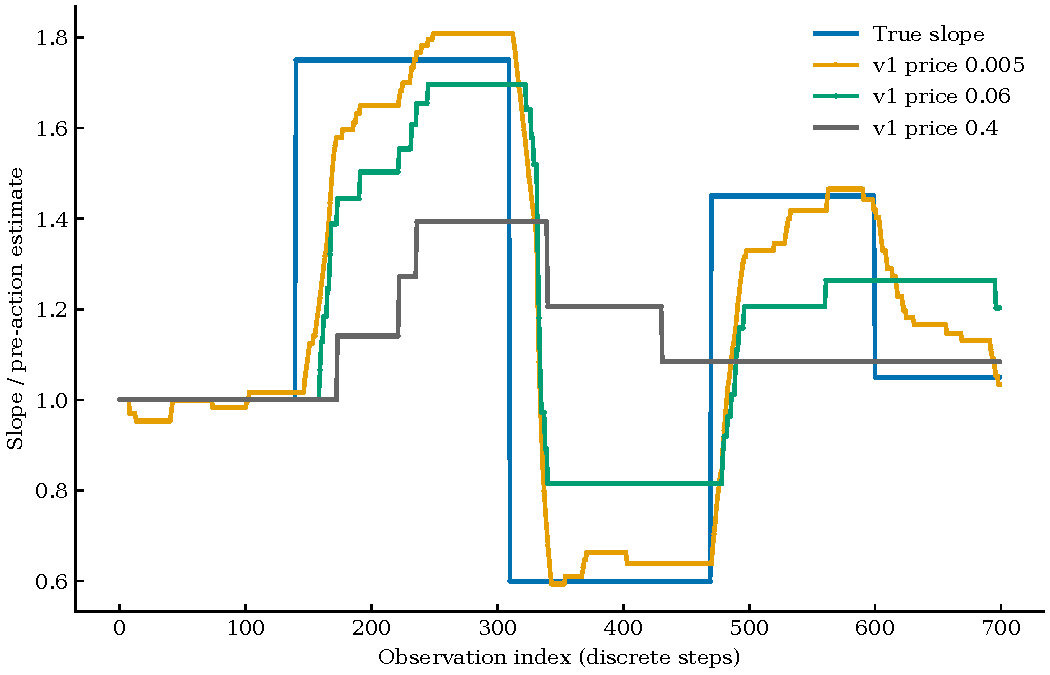
\includegraphics[width=0.88\textwidth]{figures/generated/slg-priced-policy-tracking-20261111.pdf}
\caption{Carried model state under actual-step pricing. The representative stream is seed 0, fixed before execution. The latent slope changes at observations \(140,310,470,600\) and is used only for evaluation. The other curves show the actual-step-priced rolling policy at the displayed prices. Each update moves \(0.22\) of the way towards the trailing ridge target and is bought only when \(2.5\) times its actual window improvement exceeds \(c\). Estimates are pre-action states. High prices can retain bias after a shift. This trace must be read with the matched risk, update-frequency and occupancy comparisons, not as a calibrated choice of price.}
\label{fig:num-toy-two-scale-promotion}
\end{figure*}

\subsection{Prediction risk is an external test}

Mean squared prediction error is evaluated over observations \(50,\ldots,699\), giving 650 predictions per stream. It is calculated before the current observation updates the model, rather than by rescoring the observation after fitting it. Figure~\ref{fig:prediction-risk} reports stream means at all six matched prices. The fixed-slope-1 baseline has mean error \(0.2899961\). A privileged predictor given the true slope has error \(0.0628541\), providing a noise-scale reference rather than an available policy.

The actual-step-priced policy has higher mean predictive error than the noisy-step policy at every tested matched price. At \(c=0.06\), their mean errors are approximately \(0.143405\) and \(0.121170\). The rolling control lies between them at \(0.129231\). Appendix~\ref{app:protocol} retains the full table. These observations rule out a predictive-dominance claim for this comparison. They do not contradict the action-accounting identity. That identity concerns the gain assigned to an executable candidate on an observed window, not the candidate's future predictive value.

\begin{figure*}[t]
\centering
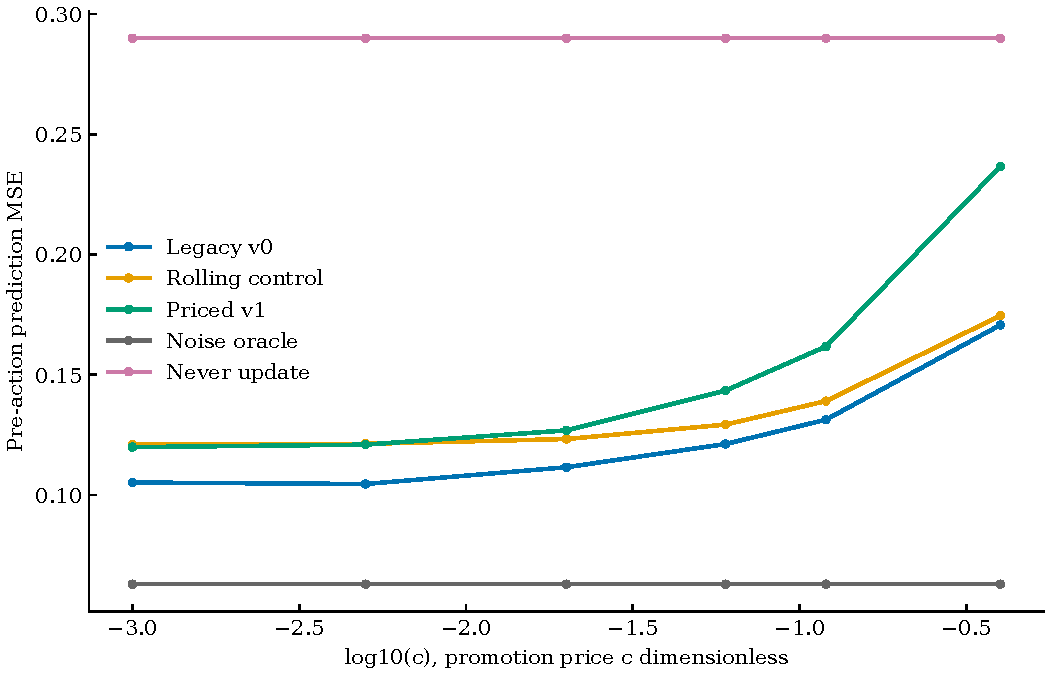
\includegraphics[width=0.84\textwidth]{figures/generated/slg-promotion-risk-20261111.pdf}
\caption{Prediction risk at matched prices. Mean squared one-step prediction error, in squared synthetic observation units, averaged over 12 matched 700-step streams using observations \(50\)--\(699\). The three methods are defined in the shared policy key in the text. The true-slope noise oracle is privileged and used only for evaluation. The never-update baseline keeps slope 1. Actual-step pricing has higher mean error than the noisy-step policy at every tested price. Lines connect the six predeclared finite stream means and carry no uncertainty bands. The complete means and the stream-level uncertainty convention are given in Appendix~\ref{app:protocol}.}
\label{fig:prediction-risk}
\end{figure*}

\subsection{Spending frequency does not measure adaptation}

The promotion fraction uses the same 650-observation window. Its numerator is the number of purchased model updates. The charged action cost per evaluated observation is \(c\) times this fraction. It does not include computation of candidates, controller maintenance or the cost of keeping a model in memory. It is a dimensionless accounting charge, not a measured energy consumption.

Figure~\ref{fig:promotion-frequency} shows the expected broad reduction in update frequency as price rises, but actual-step pricing is not always sparser than its comparators. At \(c=0.06\), the actual-step and noisy-step fractions are approximately \(0.050769\) and \(0.050385\). The actual-step policy therefore pays slightly more charged action cost while also having higher prediction error. At other prices it sometimes buys fewer updates while predicting worse. A sparse policy cannot be judged from its spending curve alone.

\begin{figure*}[t]
\centering
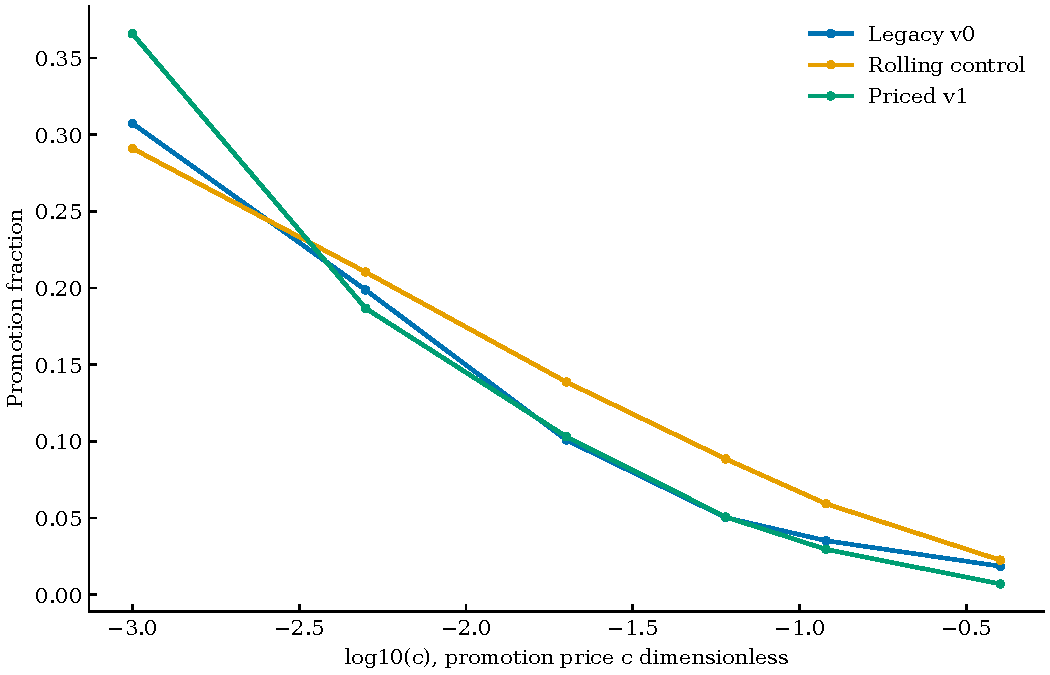
\includegraphics[width=0.84\textwidth]{figures/generated/slg-promotion-frequency-20261111.pdf}
\caption{How price changes update frequency. Promotion counts divided by 650 evaluated observations, averaged over the same 12 matched streams. Every promoted action pays the displayed dimensionless price \(c\), while staying pays zero action cost. Higher prices usually buy fewer revisions, but actual-step pricing is not always the sparsest policy. Multiplying a curve by \(c\) gives its charged action cost per evaluated observation, not total computational or physical cost. Read with Figs.~\ref{fig:prediction-risk} and \ref{fig:recovery}.}
\label{fig:promotion-frequency}
\end{figure*}

The target-occupancy test asks a different question. After a true shift, does the carried estimate enter and remain near the new target? A qualifying run consists of five consecutive pre-action estimates within \(20\%\) of the jump magnitude, entirely within the 65 observations beginning at the shift. An estimate already in band qualifies without any new update. Delay records the start of the run, not its confirmation four observations later. A shift with no qualifying run is assigned failure and a capped delay of 65.

Figure~\ref{fig:recovery} gives the fraction of shifts without such a run. Four shifts in 12 streams give 48 dependent shift evaluations per policy and price, not 48 independent experiments. At \(c=0.06\), failure fractions are \(0.1875\), \(0.270833\) and \(0.625\) for the noisy-step, rolling-control and actual-step-priced policies. Occupancy need not be monotone in price. A model that happens already to be near a later target can qualify even if it failed to react usefully to an earlier shift.

\begin{figure*}[t]
\centering
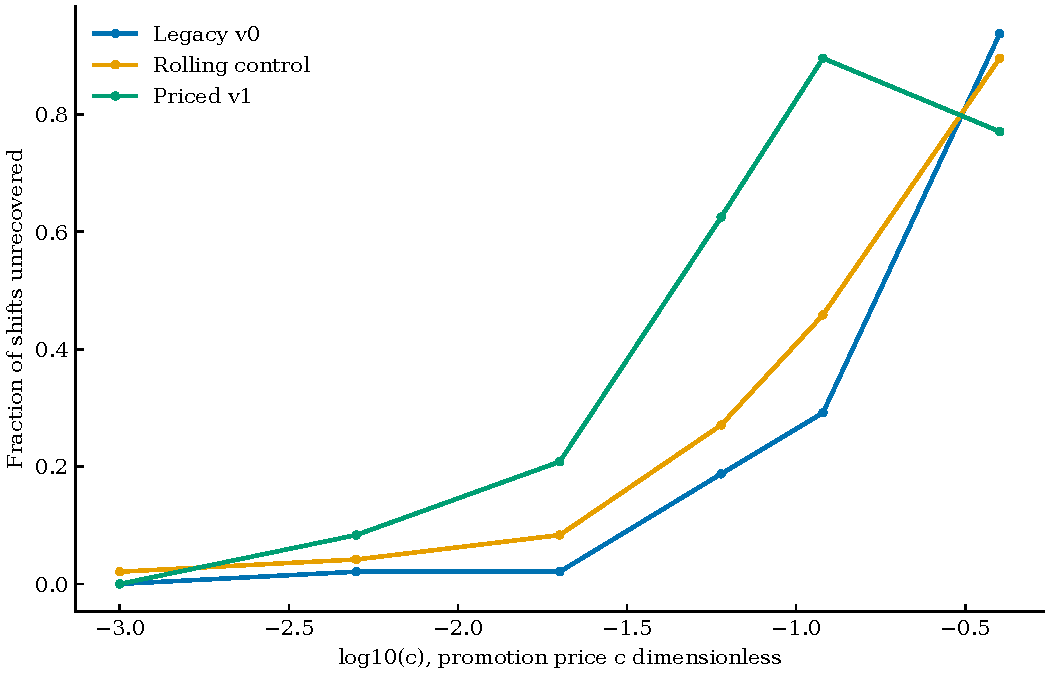
\includegraphics[width=0.84\textwidth]{figures/generated/slg-promotion-recovery-20261111.pdf}
\caption{Target occupancy after a latent shift. Fraction of shifts without five consecutive pre-action estimates in the declared band, averaged over 12 matched streams with four shifts each. The band is \(20\%\) of the jump magnitude, and the qualifying run must lie wholly within the 65-step post-shift window. Already-in-band estimates qualify without a new promotion. The criterion therefore measures occupancy, not detected change or update-caused recovery. Delay is the run start. Failures retain sentinel delay 65 in capped means. At \(c=0.06\), the three failure fractions are \(0.1875\), \(0.270833\) and \(0.625\). Lines are finite stream means without uncertainty bands.}
\label{fig:recovery}
\end{figure*}

The experiment exposes the remaining modelling task. Pricing the actual intervention prevents a mismatch between promised and executed gain. It does not tell us that an observed-window score is the right predictor of future benefit, or that a fixed price supplies adequate responsiveness after a shift. A better evaluator needs its own justified horizon, uncertainty model or parent signal. The finite results tell us where to improve the construction without discarding the accounting that makes the failure intelligible.

There is one more representational question. A receiver may not need every fine action or every step of a trace. It may ask only whether any revision occurred in a block. That is a smaller object than an adaptive trajectory. The next section derives exactly what it must retain, before asking whether a similarly small state can describe the full feedback process.

\clearpage
\section{What survives a change of representation}
\label{sec:yba-examples}

The selector assigns probabilities to fine alternatives. A receiving representation groups some of those alternatives together. We first solve that grouping problem without restricting the form of the receiving generator. Only then can we identify which additional compression loses information relevant to the event being predicted.

\subsection{Exact finite contraction}

Let \(X\) be a finite set with positive reference weights \(w_x\), let \(\pi:X\to Y\) be a surjection, and choose \(\tau>0\). For a finite generator \(K_x\), define
\begin{equation}
 \mathcal J_X(p)=\sum_xp_xK_x+
                    \tau\sum_xp_x\log\frac{p_x}{w_x}.
 \label{eq:fine-free-energy}
\end{equation}
The receiving probability is \(q_y=\sum_{\pi(x)=y}p_x\), and its inherited reference weight is \(w_y=\sum_{\pi(x)=y}w_x\). Eliminating the conditional distribution inside each fibre produces
\begin{equation}
 K_{\mathrm{eff}}(y)=
 -\tau\log\!\sum_{\pi(x)=y}\frac{w_x}{w_y}e^{-K_x/\tau}.
 \label{eq:effective-generator}
\end{equation}
The exact constrained value is
\begin{equation}
 \min_{\pi_*p=q}\mathcal J_X(p)
 =\sum_yq_yK_{\mathrm{eff}}(y)
             +\tau\sum_yq_y\log\frac{q_y}{w_y}.
 \label{eq:contraction}
\end{equation}

To see why, write \(p_x=q_yr_y(x)\) on each fibre of positive \(q_y\), and let
\(r_y^*(x)\propto w_xe^{-K_x/\tau}\) on that fibre. Collecting logarithms gives the right-hand side of Eq.~\eqref{eq:contraction} plus
\(\tau\sum_yq_yD(r_y\Vert r_y^*)\).
Each conditional relative entropy is nonnegative and can be set to zero. Fibres of zero \(q_y\) contribute nothing. Appendix~\ref{app:classical} records the complete decomposition.

The unrestricted finite free-energy family thus closes under elimination. For nested surjections, the weighted exponential sums combine associatively, so direct and staged elimination agree. A receiver using counting weights \(1\) instead of inherited weights \(w_y\) must absorb \(-\tau\log w_y\) into its generator. Omitting that adjustment changes the objective. What looks like a different effective energy can otherwise be no more than a change in the convention for counting states.

This theorem does not say that every small parametric family is closed. A quadratic, a single threshold or a generator with selected interaction terms may fail to contain the exact \(K_{\mathrm{eff}}\). That is a modelling restriction to be tested, rather than a failure of finite contraction itself.

\subsection{Independent opportunities and the OR event}

Consider a finite block \(B\) of binary update opportunities. Freeze an external margin schedule \(m_t\) and a price \(c\), then declare independent draws
\begin{equation}
 U_t\sim\operatorname{Bernoulli}(p_t),\qquad
 p_t=\sigma(m_t-c),\qquad t\in B .
 \label{eq:num-toy-fine-promotion}
\end{equation}
The reference mass ratio and statistical scale have been fixed to the equal-mass, unit-scale two-action convention. This is a product ensemble on a supplied schedule. It is not obtained merely by conditioning an adaptive learner on its realised margin path. Such a path can encode earlier actions and therefore carries selection information.

The receiver asks only whether any fine event occurred:
\[
 N_B=\sum_{t\in B}U_t,\qquad U_B=\mathbf1\{N_B\geq1\}.
\]
Independence gives
\begin{equation}
 q_B=\Pr(U_B=1)=1-\prod_{t\in B}(1-p_t)
                =1-e^{-h_B(c)},
 \label{eq:num-toy-pushed-probability}
\end{equation}
where the cumulative hazard is
\begin{equation}
 h_B(c)=-\sum_{t\in B}\log(1-p_t)
       =\sum_{t\in B}\log(1+e^{m_t-c}).
 \label{eq:hazard}
\end{equation}
For independent disjoint blocks,
\(h_{A\cup B}=h_A+h_B\).
The retained event statistic is additive and its merging is associative. The OR event closes exactly in hazard.

The same result is a fibre contraction. A path \(\mathbf u\) has weight
\(\exp[\sum_tu_t(m_t-c)]\), with partition sum
\[
 Z_B=\prod_t(1+e^{m_t-c})=e^{h_B}.
\]
The all-zero fibre weighs 1. The nonempty fibre weighs \(Z_B-1\). With counting reference on the two receiving states, their effective generators are \(H_0=0\) and
\(H_1=-\log(e^{h_B}-1)\).
The resulting binary Gibbs probability is exactly Eq.~\eqref{eq:num-toy-pushed-probability}. Keeping the event does not require keeping every path.

\subsection{The error of a smaller receiving description}

Suppose the receiver keeps only the summed margin
\(S_B=\sum_tm_t\) and insists on a logistic law
\(\widehat q_B=\sigma(S_B-a)\) with one common intercept \(a\). Each individual block can be represented exactly using
\begin{equation}
 c_{\mathrm{eff}}(B;c)
 =S_B-\operatorname{logit}q_B,\qquad
 \operatorname{logit}q=\log\frac q{1-q}.
 \label{eq:num-toy-running-cost}
\end{equation}
But this intercept generally depends on the margin pattern, not only its sum.

For two margins \(m+\delta,m-\delta\), the nonempty path weight is
\begin{equation}
 2e^{m-c}\cosh\delta+e^{2(m-c)} .
 \label{eq:heterogeneous-pair}
\end{equation}
The summed margin remains \(2m\), while the first term changes with \(\delta\). The equal-sum pairs \((0.1,0.1)\) and \((0.7,-0.5)\), at \(c=0.5\), differ in OR probability by approximately \(0.0293292\). A summed margin and a shared intercept cannot distinguish them. Hazard can.

For a collection of blocks, choosing
\(\bar c_{\mathrm{eff}}\) as the arithmetic mean of the exact block intercepts minimises squared intercept error, equivalently squared log-odds error. It is not claimed to minimise total variation or relative entropy. For Bernoulli distributions, total variation is the absolute probability difference. Since the logistic derivative is at most \(1/4\),
\begin{equation}
 |q_B-\sigma(S_B-\bar c_{\mathrm{eff}})|
 \leq \frac14|c_{\mathrm{eff}}(B;c)-\bar c_{\mathrm{eff}}|.
 \label{eq:tv-bound}
\end{equation}
This is a bound on disagreement about the retained event. It is not a claim to measure all Shannon information lost from a fine trajectory.

Figure~\ref{fig:num-toy-coarse-defect}(a) applies these descriptions to four predeclared blocks of four margins over 81 prices. Exact hazard agrees with OR to floating-point precision. A common intercept substantially reduces the naive same-price error, but leaves a residual because the blocks are heterogeneous. The four schedules and all averaging conventions are supplied in Appendix~\ref{app:or-protocol}.

\subsection{What the threshold response counts}

Holding all fine margins fixed, differentiate Eq.~\eqref{eq:hazard}:
\[
 \frac{dh_B}{dc}=-\sum_tp_t,\qquad
 \frac{d\,\operatorname{logit}q_B}{dc}
                           =-\frac{\sum_tp_t}{q_B}.
\]
It follows that
\begin{align}
 \frac{dc_{\mathrm{eff}}}{dc}
 &=\frac{\sum_tp_t}{q_B}
 =\mathbb E[N_B\mid N_B\geq1],\nonumber\\
 1&\leq\frac{dc_{\mathrm{eff}}}{dc}\leq|B|.
 \label{eq:multiplicity}
\end{align}
For finite logistic probabilities and \(|B|>1\), both bounds are strict. The receiver's threshold sensitivity counts how many fine events tend to underlie a nonempty block. Figure~\ref{fig:num-toy-coarse-defect}(b) displays that quantity for the same schedules.

\begin{figure*}[p]
\centering
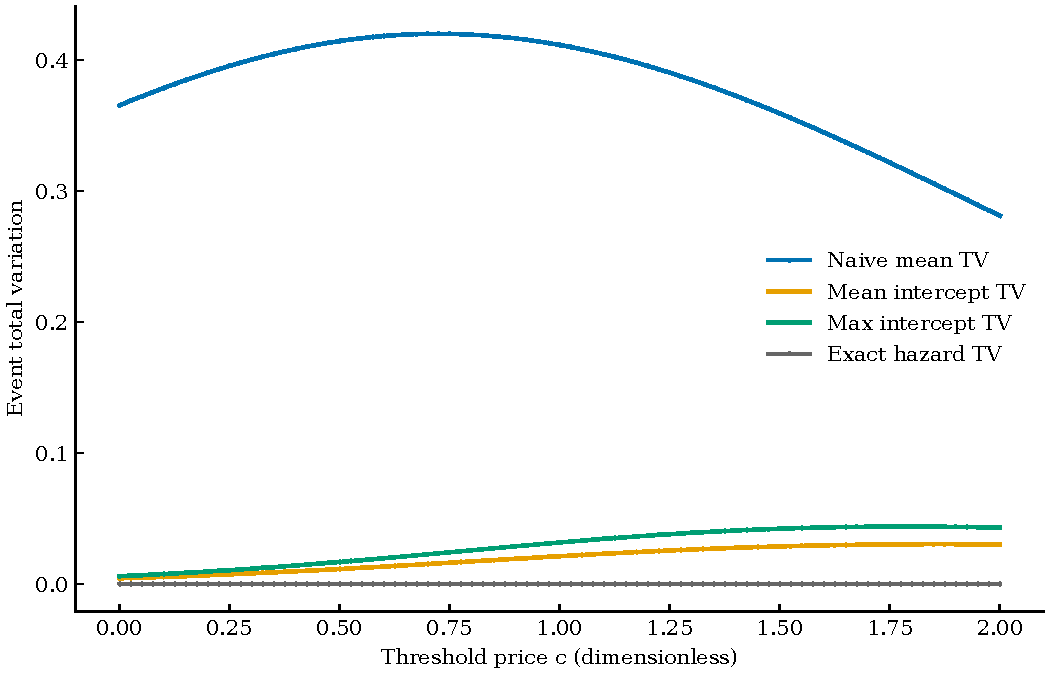
\includegraphics[width=0.70\textwidth]{figures/generated/slg-or-hazard-defect-20261111.pdf}\\[1ex]
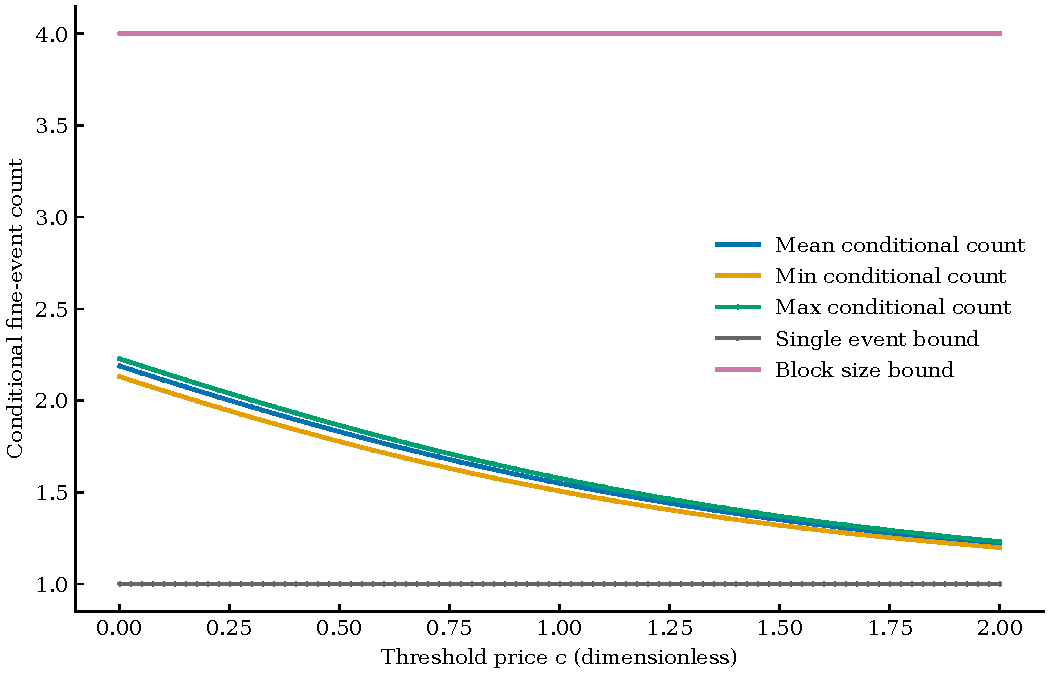
\includegraphics[width=0.70\textwidth]{figures/generated/slg-or-event-multiplicity-20261111.pdf}
\caption{Exact event closure and the cost of a smaller description. Top (a): Bernoulli event total variation over four externally frozen independent four-event schedules at 81 prices. Exact hazard retains \(h_B(c)\) and reproduces the OR probability. The naive law uses \(\sigma(S_B-c)\). The common-intercept law uses the arithmetic mean of block-specific \(c_{\mathrm{eff}}\) at each price. Its mean and maximum residuals quantify the effect of that restriction. The mean intercept minimises squared log-odds error, not TV. Bottom (b): for the same blocks, \(dc_{\mathrm{eff}}/dc=\mathbb E[N_B\mid N_B\geq1]\). Curves give its block mean, minimum and maximum, with exact bounds 1 and 4. This is conditional event multiplicity, not an instability eigenvalue. The full margin schedules are retained for repricing. A single hazard value at one price is insufficient for that response.}
\label{fig:num-toy-coarse-defect}
\end{figure*}

A slope above one therefore needs no critical or unstable mechanism. No iterated rescaled coupling transformation or fixed point has been defined here from which an RG eigenvalue could be extracted. Similarly, a negative effective intercept is an event log-odds offset produced by multiple opportunities, not negative physical work.

The dependence on price exposes another distinction. One number \(h_B(c_0)\) is sufficient for the OR probability at \(c_0\). It does not determine the entire function \(h_B(c)\), or even its derivative at \(c_0\). Repricing requires a richer retained description, such as the complete frozen margin schedule. Sufficiency is always relative to a question.

\subsection{Receiving dynamics requires more than event closure}
\label{subsec:receiving-dynamics}

For an actual adaptive learner, the current state and history determine the next margins. The appropriate object is its transition kernel or vector field, not an independent product law substituted along a realised trace. Exact aggregation of one event does not prove that a coarse state supports a closed adaptive process.

Let \(P(x,\cdot)\) be a finite-state fine Markov kernel, \(\pi:X\to Y\) a state map, and \(Q(y,\cdot)\) a proposed receiving kernel. Define total variation on their common receiving support by
\[
 \|\mu-\nu\|_{\mathrm{TV}}
       =\frac12\sum_{y\in Y}|\mu(y)-\nu(y)|.
\]
A one-step defect is
\begin{equation}
 \epsilon=
 \sup_{x\in X}
 \|\pi_*P(x,\cdot)-Q(\pi x,\cdot)\|_{\mathrm{TV}} .
 \label{eq:kernel-defect}
\end{equation}
Exact closure requires the pushed transition law to be identical for every fine state in a fibre. If initial coarse laws agree, the discrepancy after \(n\) steps is bounded by \(\min(1,n\epsilon)\). This bound uses TV contraction under a Markov kernel, not an assumption that the omitted variables cease to matter.

For smooth deterministic dynamics, let \(v\) be the fine field, \(w\) the receiving field, and \(\pi\) a differentiable map. The local mismatch is
\begin{equation}
 \delta(x)=\|D\pi_xv(x)-w(\pi x)\|.
 \label{eq:yba-app-infinitesimal-defect}
\end{equation}
The norm, domain and time window are part of the test. If \(\delta(x)\leq\delta_0\) along the trajectories and \(w\) is \(L\)-Lipschitz on a domain containing both compared paths, their initially equal coarse states remain within
\(\delta_0(e^{Lt}-1)/L\), with limit \(\delta_0t\) for \(L=0\). Appendix~\ref{app:maps} derives both receiving bounds.

Coordinate changes and coarse-graining should not be conflated. An invertible smooth coordinate map transports the complete field by the chain rule. A many-to-one map discards state. It can destroy autonomous dynamics even when all fine equations are correct. Restoring closure may require memory or another retained statistic rather than a different microscopic law. The OR calculation gives a concrete instance of finding the useful statistic instead of declaring every discrepancy a failure of learning.

\clearpage
\section{Primary methods and the present construction}
\label{sec:yba-background}

The preceding derivations use standard statistical machinery for a particular model-revision problem. Jaynes' maximum-entropy construction gives an exponential distribution when a finite set of alternatives is assigned moment constraints, with the partition function normalising the result \cite{jaynes1957information}. In Section~\ref{sec:self-consistent-loss-geometry}, the corresponding premise is stated directly as a relative-entropy objective with a reference measure. The new work is not the exponential form. It is the specification of executed candidate actions, their common horizon and their coupling to an evaluator that is itself part of the state.

The reference measure matters twice. It determines how many alternatives a score represents, and it supplies the inherited weights in exact contraction. A regulariser cannot be declared uniquely necessary merely because its chosen finite family closes. We have proved the conditional-KL identity for the stated objective. An axiomatic characterisation of all permissible inference rules is a separate claim and is not needed for the calculations here.

Multitask learning supplies the natural setting for shared representations. In Caruana's construction, several task outputs train a common hidden layer, so training information for one task can improve another through learned features \cite{caruana1997multitask}. Our two-target register does not reproduce that generalisation mechanism. It isolates the cost of imposing distinct demands on one state and adds a priced alternative partition. The connection is useful because it separates shared representation as a source of transfer from the decision to preserve or alter a particular sharing arrangement.

The geometry of an update also requires an explicit convention. On a smooth model manifold with positive metric tensor \(g(M)\), steepest descent of a scalar evaluator has coordinate form
\begin{equation}
 \dot M=-g(M)^{-1}\nabla_M\mathcal L(M,\lambda).
 \label{eq:yba-natural-flow}
\end{equation}
Transforming coordinates consistently transports the metric and vector field. Resetting the metric to the identity after a nonlinear coordinate change instead defines a different motion. This distinction underlies the receiving-map tests: transporting a motion and discarding state are different operations.

The quantum extension identifies where the classical analogy genuinely stops. Quantum relative entropy is monotone under a quantum channel, and equality is characterised by recovery with the appropriate reference and support conventions \cite{PETZ200347a4ef,Junge20189e4744}. Appendix~\ref{app:quantum} applies that result to constrained elimination. An equilibrium marginal generator always reproduces the marginal of its Gibbs state. It need not give the constrained variational value at every prescribed marginal. Feasible recovery, rather than formal similarity to a classical sum, is the equality condition.

These connections place the contribution at the level of a calculable regulator architecture. The framework combines finite action accounting, endogenous evaluator state, a partition purchase and explicit receiving tests. It does not derive a universal biological loss from maximum entropy, or infer dynamical closure from a statistical boundary. The formal choices are visible enough to be altered and compared.

\section{Consequences for a learner that can revise its representation}
\label{sec:yba-discussion}

The register at the beginning could move, arbitrate or split. We can now say what distinguishes those operations. Register motion reduces a task score at a fixed authority. Arbitration redistributes whose error can move the same substrate. Splitting changes which demands must share a state. The common ledger supplies an exact boundary at which the last operation pays. The boundary would be invisible to a model that allowed only weight changes.

An endogenous evaluator introduces a further state. Our explicit reuse-mode controller shows that its authority coordinate can converge together with the model under stated conditions. It does not implement or establish convergence of a capacity-purchase mechanism. The purchase boundary remains a static comparison, and the tracking policies use their own fixed scoring rule. The damping, coupling, parent drive and update order carry the reuse-mode result. A switched architecture with a learning parent must include those additional states in its own analysis.

The tracking evidence then separates coherent accounting from a successful evaluator. Actual-step pricing assigns the executed move its actual observed-window gain and propagates its state correctly. Yet it predicts worse than the noisy-step comparator at every matched price in the retained experiment. The productive conclusion is not that cost accounting should be abandoned. It is that the evaluator's horizon and statistical assumptions remain design questions. A policy can reliably buy what it scored while scoring the wrong thing for tomorrow's prediction.

The representation calculation suggests how to make those questions precise. OR aggregation preserves the event exactly if the receiver retains cumulative hazard. Summed margins with one common intercept lose a particular distinction between blocks. Their residual TV measures disagreement about the event. Repricing asks a richer question and needs more than one hazard value. Adaptive evolution asks a richer question again and requires a state or history kernel. Each enlargement is motivated by an operation the smaller representation cannot support.

This gives a practical interpretation of the proposed three laws. Endogenous evaluation asks where the score comes from and how it changes. Embodied price asks which transition is purchased, on which ledger and horizon. Representation covariance asks which map, observable or transition is to survive, at what tolerance. A complete answer need not be exact at every scale. It must make the approximation and the receiving question explicit.

Several comparisons now become possible without invoking a universal theory of intelligence. Hold task losses fixed and compare a weight-only controller with one that can purchase an additional register at a declared price. Hold executable actions fixed and compare observed-window gain with a forecast-based or uncertainty-sensitive evaluator. Hold fine dynamics fixed and compare receiving descriptions with and without retained history. In each case the extra operation has an explicit cost and an explicit consequence to measure.

The nested construction also gives a disciplined use for attention-like arbitration and finite self-modelling. Authority weights can route error among competing demands without creating capacity. A represented self-state can help a controller predict its own subsequent operation without requiring unlimited recursion. Whether either mechanism pays in a particular organism or engineered system is a question about its actual signals, resources and task. The finite framework supplies candidate measurements, not a biological guarantee or a clinical diagnosis.

The most useful next step is therefore not to announce that all learning minimises one hidden scalar. It is to build models in which the alternatives are genuine: a move that is executed as priced, an evaluator that can be perturbed, a partition whose purchase changes the feasible states, and a receiving representation whose predictions can be compared. Self-consistent loss geometry names the coupled object that remains when these choices are made explicit. Its scientific value lies in the calculations and failures those choices let us expose.

\appendix
\section{The finite action protocol}
\label{sec:yba-appendix}
\label{app:actions}

For the finite selector, set \(K_u=C_u-\beta G_u\) and
\(r_u=\mu_ue^{-K_u/\tau}/Z\). Substitution gives
\begin{align}
 \Phi(P)
 &=\tau\sum_uP_u\log\frac{P_u}{r_u}-\tau\log Z .
 \label{eq:selector-proof}
\end{align}
Nonnegativity of relative entropy gives the unique minimiser \(r\). Positive \(\mu_u\), finite \(K_u\), a finite action set and \(\tau>0\) ensure full support. Hard exclusions should instead be represented by removing unavailable actions or restricting support explicitly. They are not part of the positive-mass proof.

The deterministic policy used in the tracking calculation compares \(\beta G_u-C_u\) for two equal-reference-mass actions and uses strict inequality to buy an update. Its score is not a statement that an action was sampled. A different tie rule changes a deterministic transition at equality and must be retained with the state protocol.

The actual trailing window is
\(D_t=\{\max(0,t-27),\ldots,t\}\).
For a generic target displacement \(v\), direct expansion of
\((y_i-(\vartheta+\rho v)x_i)^2\) gives Eq.~\eqref{eq:partial-gain}. At the unregularised least-squares target,
\(B_t-A_t\vartheta=A_tv\), so
\(G_{\mathrm{partial}}=(2\rho-\rho^2)A_tv^2\).
The full-fit gain is \(A_tv^2\). A ridge target does not satisfy that first equality exactly.

Finite branch controls used constant observations \(x_i=1,y_i=0.8\), the same partial-step scorer, and the same strict selection/application path. At price \(0.02\), an eight-observation call promotes from 1 to \(0.9559999780000028\). A nine-observation call reusing the actual carried state promotes to \(0.9216799632844488\). At price \(0.06\), the eight-observation call stays. At the positive executable tie price \(0.039160017159996584\), recomputed binary64 scores are exactly equal and the policy stays.

An independent rational oracle uses
\[
 \vartheta_{\mathrm w}=\frac{n(4/5)}{n+1/10^6},\quad
 \vartheta_1=\vartheta+\frac{11}{50}(\vartheta_{\mathrm w}-\vartheta),
\]
and \(G_1=2\delta(4/5-\vartheta)-\delta^2\), with
\(\delta=\vartheta_1-\vartheta\).
The largest recorded state/gain/score residual in the four-case control was \(6.25\times10^{-17}\), below the predeclared \(10^{-12}\) tolerance. An exact floating-point score tie is a branch observation, not an assertion that binary arithmetic equals its rational idealisation.

\section{Proof of weighted classical contraction}
\label{app:classical}

For a positive receiving mass \(q_y\), write
\(p_x=q_yr_y(x)\) on \(\pi^{-1}(y)\). Define
\[
 Z_y=\sum_{\pi(x)=y}w_xe^{-K_x/\tau},
 \qquad r_y^*(x)=\frac{w_xe^{-K_x/\tau}}{Z_y}.
\]
Since \(K_{\mathrm{eff}}(y)=-\tau\log(Z_y/w_y)\),
\begin{align}
 \mathcal J_X(p)
 ={}&\sum_yq_yK_{\mathrm{eff}}(y)
       +\tau\sum_yq_y\log(q_y/w_y)\nonumber\\
    &+\tau\sum_yq_yD(r_y\Vert r_y^*).
 \label{eq:conditional-kl}
\end{align}
Zero-mass fibres contribute zero under \(0\log0=0\). All other conditional relative entropies can be minimised independently. This proves Eq.~\eqref{eq:contraction} without an assumption about how a dynamical learner explores the fibre.

For a further surjection \(\psi:Y\to Z\), let
\(w_z=\sum_{\psi(y)=z}w_y\). Then
\begin{align}
 &\sum_{\psi(y)=z}\frac{w_y}{w_z}e^{-K_{\mathrm{eff}}(y)/\tau}
 \nonumber\\
 &\hspace{1em}=
 \sum_{(\psi\circ\pi)(x)=z}\frac{w_x}{w_z}e^{-K_x/\tau}.
 \label{eq:staged-contraction}
\end{align}
Direct and staged elimination therefore agree. A change in reference convention must be included before comparing generators. Restricted parametrisations and repeated projection back into them are additional operations and need not preserve this associativity.

\section{Convergence of the reuse-mode controller}
\label{app:controller}

Each component of Eq.~\eqref{eq:regulator} is a convex combination of values in \([-1,1]\), so the square is invariant. For two states at a common frozen \(h\), the Lipschitz property of \(\tanh\) gives
\begin{align*}
 |\delta m^+|&\leq(1-a_m)|\delta m|+a_m|\delta\lambda|,\\
 |\delta\lambda^+|/\nu
 &\leq(1-a_\lambda)|\delta\lambda|/\nu
             +(a_\lambda k/\nu)|\delta m|.
\end{align*}
Taking the weighted maximum gives the factor \(r<1\) in Eq.~\eqref{eq:contraction-factor}. The closed square is complete in this norm. The contraction theorem supplies a unique fixed point and the geometric bound
\(\|z_n-z^*\|_\nu\leq r^n\|z_0-z^*\|_\nu\).
An uncontractive continuous self-map of a compact convex state domain may still have a fixed point, but continuity alone does not supply attraction.

The parameter restriction \(k<1\) is sufficient, not a theorem that all larger couplings fail. A switched register or changing \(h\) is a different problem. The retained finite checks corroborate examples of this fixed-drive map, not every parent-learning extension.

Suppose a specified external improvement field in the same model metric is \(g_{\mathrm{ext}}\). Exact alignment
\(-\operatorname{grad}_m J=g_{\mathrm{ext}}\) is an additional premise. At a stationary gradient-model state it implies \(g_{\mathrm{ext}}=0\). With alignment defect at most \(\varepsilon\), stationarity bounds \(\|g_{\mathrm{ext}}\|\) by \(\varepsilon\). A fixed-point equation alone provides neither premise. On a neighbourhood, representing a prescribed field by a scalar loss also requires the relevant integrability conditions.

\section{The OR figure protocol}
\label{app:or-protocol}

Under the declared independent product law, summing binary path weights gives \(Z_B=e^{h_B}\). The empty path weighs 1, so the nonempty probability is \((Z_B-1)/Z_B\). Its log odds are \(\log(e^{h_B}-1)\). Differentiating at fixed margins gives
\[
 \frac{dh_B}{dc}=-\sum_tp_t,\qquad
 \frac{d\,\operatorname{logit}q_B}{dc}
                  =-\frac{\sum_tp_t}{q_B}.
\]
Because \(N_B=0\) on the empty event,
\(\mathbb E N_B=q_B\mathbb E[N_B\mid N_B\geq1]\).
This proves Eq.~\eqref{eq:multiplicity}. For more than one finite logistic opportunity, both one event and multiple events have positive conditional probability, giving the strict bounds.

The four externally frozen margin blocks in Fig.~\ref{fig:num-toy-coarse-defect} are the rows of
\[
 \begin{pmatrix}
 -0.4&0.2&0.9&-0.1\\
 0.1&0.1&0.1&0.1\\
 0.7&-0.5&0.7&-0.5\\
 -0.2&-0.2&0.2&0.2
 \end{pmatrix}.
\]
The 81 equally spaced prices run from \(0.001\) to 2 inclusive. At each price, the naive law uses \(\sigma(S_B-c)\). The restricted fitted law uses the arithmetic mean of the four exact block intercepts. Mean TV averages the four absolute event-probability errors. Maximum TV takes their maximum. Multiplicity curves give the mean, minimum and maximum of \(\sum_tp_t/q_B\) over blocks.

The numerical implementation uses stable softplus and exponential expressions in double precision. The maximum recorded difference between exact hazard and the OR product was \(2.220446049250313\times10^{-16}\). This is numerical agreement with an algebraic identity. It is not an observed instability threshold or a fit to the adaptive tracking process.

The full function \(h_B(c)\), rather than one number \(h_B(c_0)\), is available for repricing because the margin schedules are retained. Replacing every block by the mean intercept is a projection. Repeating that projection after regrouping blocks need not reproduce direct elimination, even though exact hazard merging is associative.

\section{Bounds for receiving dynamics}
\label{app:maps}

For a differentiable receiving map \(\pi\), write \(x(t)\) for the fine trajectory and \(y(t)\) for the proposed receiving trajectory, with \(y(0)=\pi x(0)\). Suppose both remain in a declared receiving domain for \(0\leq t\leq T\), that \(w\) is \(L\)-Lipschitz there, and that
\(\|D\pi_xv(x)-w(\pi x)\|\leq\delta_0\) along the relevant fine paths. Adding and subtracting \(w(\pi x(t))\) gives
\[
 \|\pi x(t)-y(t)\|
 \leq\int_0^t[\delta_0+L\|\pi x(s)-y(s)\|]\,ds .
\]
Gronwall's inequality yields
\[
 \|\pi x(t)-y(t)\|\leq
 \begin{cases}
 \delta_0(e^{Lt}-1)/L,&L>0,\\
 \delta_0t,&L=0 .
 \end{cases}
\]
The metric cannot be changed midway through the comparison. For invertible coordinate maps, consistent field transport makes the local mismatch vanish. A coarse map need not admit any autonomous field \(w\) with zero mismatch.

For finite kernels, let \(\mu_n\) be the fine law and \(\nu_n\) the proposed receiving law, with \(\nu_0=\pi_*\mu_0\). The uniform defect in Eq.~\eqref{eq:kernel-defect} implies
\[
 \|\pi_*(\mu_nP)-(\pi_*\mu_n)Q\|_{\mathrm{TV}}\leq\epsilon .
\]
Adding and subtracting \((\pi_*\mu_n)Q\), then using TV contraction under \(Q\), gives
\(d_{n+1}\leq\epsilon+d_n\).
Consequently \(d_n\leq\min(1,n\epsilon)\). This is a worst-case finite-horizon statement. A smaller averaged defect requires its own state distribution and does not automatically imply the uniform bound.

\section{Logarithmic capacity costs}
\label{app:rank}

A multiplicative capacity coordinate gives a useful special case of the price ledger. Suppose
\(f:\mathbb N\to\mathbb R_{\geq0}\) is nondecreasing and obeys
\(f(rs)=f(r)+f(s)\).
Then \(f(1)=0\). If \(f(2)=0\), bounding any \(n\) by a power of two forces \(f(n)=0\). Otherwise put \(k_j=\lfloor j\log_2n\rfloor\). Monotonicity gives
\[
 k_jf(2)\leq jf(n)\leq(k_j+1)f(2).
\]
Dividing by \(j\) and taking the limit proves
\(f(n)=\kappa\log n\), with \(\kappa=f(2)/\log2\geq0\).
The composition premise concerns a declared capacity label. It is not implied by statistical independence of probability-order ranks.

For example, marginal probabilities \((0.7,0.3)\) and \((0.6,0.4)\) produce joint probabilities \(0.42,0.28,0.18,0.12\). The pair with marginal ranks \(2,1\) has joint probability-order rank 3, not their product 2. If labels are instead explicitly multiplicative capacities, their multiplicities remain in the reference measure. Write \(I>0\) for the inverse statistical cost scale when the cost is \(\log r\). Two factors labelled \(\{1,2\}\) produce \(\{1,2,2,4\}\), so their cost-weighted partition sum is \((1+2^{-I})^2\).

A separate consecutive-label model has one alternative at each \(r=1,\ldots,R\). With equal reference masses, equal gains, cost \(\log r\) and inverse cost scale \(I\), the selector specialises to
\[
 p_I(r)=\frac{r^{-I}}{Z_R(I)},\qquad
 Z_R(I)=\sum_{r=1}^Rr^{-I}.
\]
This follows from the stated maximum-entropy or relative-entropy selection premise, not from a universal empirical rank law. Its response satisfies
\[
 -\partial_I\log Z_R=\mathbb E_I\log r,\qquad
 \partial_I^2\log Z_R=\operatorname{Var}_I(\log r).
\]
The infinite consecutive-label limit is normalised by \(\zeta(I)\) only for \(I>1\). Finite representational systems keep their actual cutoff and multiplicities.
\section{A finite comparison of priced update policies}
\label{app:protocol}

Twelve predeclared streams, seeds \(0,\ldots,11\), each contain 700 observations indexed \(0,\ldots,699\). Inputs are independent standard normal draws and \(y_t=\vartheta_t^*x_t+\xi_t\), with independent Gaussian noise of standard deviation \(0.25\). The true slope starts at 1 and becomes \(1.75,0.6,1.45,1.05\) at observations \(140,310,470,600\). Each seed's observations are reused for all three policies and prices \(c\in\{0.001,0.005,0.02,0.06,0.12,0.4\}\). States start at 1. The 216 trajectories comprise 150984 decisions. Parameters are \(\beta=2.5\), window length 28, minimum eight fit points, ridge denominator \(10^{-6}\), partial step \(0.22\). No price is selected as an optimum.

We define the three mechanisms once. The \emph{full-fit-scored noisy-step policy} scores \(G_{\rm full}=\max(0,J_t(\vartheta)-J_t(\vartheta_{\mathrm w}))\) against proxy \(g_0=0.1\min((y_t-\vartheta x_t)^2,0.25^2)\), but applies a partial step towards \(\operatorname{clip}(y_t/x_t,-1.5,3.5)\), falling back to the rolling fit when \(|x_t|\leq0.15\). The \emph{full-fit-scored rolling control} uses that full-fit/proxy scoring but applies the partial rolling-fit action of Eq.~\eqref{eq:actions}. The \emph{actual-step-priced rolling policy} scores that actual candidate directly and gives staying zero gain. Each buys an update iff its declared \(\beta(G_1-G_0)>c\), pays \(c\), and otherwise carries the unchanged state. The first two policies' positive proxy is not a realised no-update improvement. The rolling control isolates action-target change from the combined repricing of the partial step and staying baseline.

Prediction uses the state available \emph{before} the current observation updates it. Mean squared prediction error and promotion fractions use \(t=50,\ldots,699\), hence 650 observations per stream. Charged cost per evaluated observation is \(c\) times promotion fraction. It excludes controller computation and maintenance and is not measured energy. A fixed-slope-1 baseline and privileged true-slope predictor have mean errors \(0.2899961\) and \(0.0628541\). Truth is used only for evaluation. Table~\ref{tab:policies} retains all six matched prices. Actual-step pricing has higher mean error than the noisy-step policy throughout. At \(c=0.06\), it also has essentially the same, slightly higher charged cost. At some other prices it buys fewer updates while predicting worse. Internal gain accounting supplies no dominance conclusion.

\begin{table*}[t]
\centering
\caption{Matched synthetic comparison. N, R and A denote the full-fit-scored noisy-step policy, full-fit-scored rolling control and actual-step-priced rolling policy defined in Appendix~\ref{app:protocol}. Entries average 12 streams. Promotion fraction is updates/650. Failure averages each stream's four-shift fraction without a qualifying in-band run. These are descriptive means, not an optimum or independent-shift uncertainty estimate.}
\label{tab:policies}
\begin{tabular}{c|ccc|ccc|ccc}
\hline
&\multicolumn{3}{c|}{Prediction MSE}&\multicolumn{3}{c|}{Promotion fraction}&\multicolumn{3}{c}{Unrecovered fraction}\\
\(c\)&N&R&A&N&R&A&N&R&A\\ \hline
0.001&0.105146&0.120979&0.119865&0.307308&0.291026&0.365769&0&0.020833&0\\
0.005&0.104527&0.121233&0.120905&0.198718&0.210385&0.186795&0.020833&0.041667&0.083333\\
0.02&0.111496&0.123236&0.126844&0.100897&0.138718&0.103077&0.020833&0.083333&0.208333\\
0.06&0.121170&0.129231&0.143405&0.050385&0.088590&0.050769&0.187500&0.270833&0.625000\\
0.12&0.131270&0.139036&0.161741&0.035256&0.059359&0.029615&0.291667&0.458333&0.895833\\
0.4&0.170679&0.174570&0.236637&0.018590&0.022564&0.007051&0.937500&0.895833&0.770833\\ \hline
\end{tabular}
\end{table*}

At a true shift \(s\), a qualifying run is five consecutive pre-action estimates within \(20\%\) of the jump magnitude, entirely inside \([s,s+65)\). Delay is the first run's \emph{start}, not confirmation four observations later. Already-in-band estimates qualify without a new promotion. Thus recovery measures target occupancy, not detected change or update-triggered success. Without a qualifying run, the shift fails and sentinel delay 65 remains in the capped-delay mean. Four shifts in 12 streams give 48 dependent evaluations per policy/price. Occupancy need not be monotone in price: a model already near the last target can qualify without reacting successfully to preceding shifts.

An off-transition frequency excludes the four nonoverlapping 65-step post-shift windows, leaving 390 evaluated observations per stream. Its denominator is 390, not the number of promotions, and it is not a false-positive probability. Each mean averages 12 stream-level quantities. Descriptive SE is the sample standard deviation divided by \(\sqrt{12}\). Paired comparisons subtract same-seed errors before computing SE. No binomial uncertainty based on 48 independent shifts is used. Realised gains on overlapping windows cannot be summed into additive forecast improvement.

Reference controls matched six seed-0 noisy-step trajectories to the original policy and three predeclared seed-0 actual-step trajectories to the selection/application implementation, with recorded zero state discrepancy and identical choices under tolerance \(10^{-12}\). Actual-step candidate-versus-realised accounting discrepancy was zero on recorded paths. These controls establish finite implementation agreement, whereas the observations establish the finite predictive comparison. The executed calculations used Python 3.14.7 and NumPy 2.5.1. No new scientific run was made to produce this manuscript.


\subsection{Updates outside post-shift windows}

Figure~\ref{fig:off-transition} asks where revisions are spent outside the post-shift windows. Excluding the four nonoverlapping 65-step post-shift windows from the 650-observation evaluation interval leaves 390 observations per stream. The off-transition rate is purchased updates in those observations divided by 390. It is not the share of promotions that were false, and it is not a false-positive probability. Useful adaptation to noisy observations can occur between the designated latent shifts.

\begin{figure*}[t]
\centering
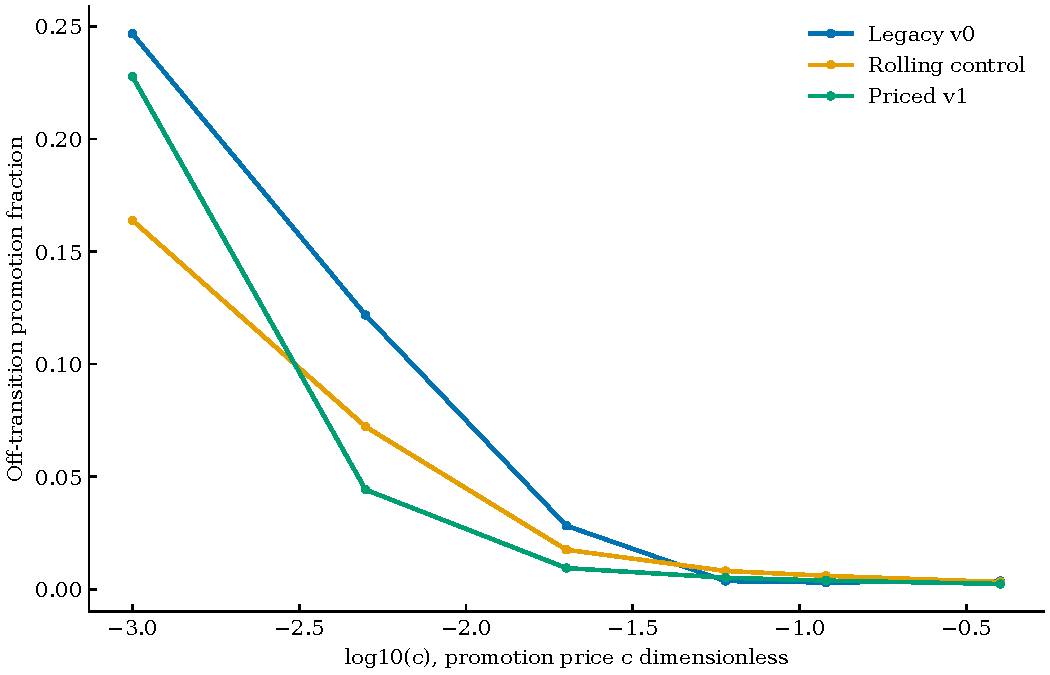
\includegraphics[width=0.84\textwidth]{figures/generated/slg-off-transition-promotions-20261111.pdf}
\caption{Updates outside the declared post-shift windows. Promotion fraction over observations \(50\)--\(699\) excluding each interval \([s,s+65)\) beginning at a true shift \(s\), averaged over 12 matched streams. The denominator is 390 observations per stream, not the number of updates. The same three methods and prices are used as in the main comparison. This operational rate is not a false-positive probability. Read with prediction risk and target occupancy before treating suppressed updates as improved adaptation. Lines show finite stream means without uncertainty bands.}
\label{fig:off-transition}
\label{fig:slg-off-transition-promotions-20261111}
\end{figure*}

\section{Quantum contraction as feasible recovery}
\label{app:quantum}

The classical fibre proof relies on the possibility of choosing conditional distributions independently at a fixed marginal. Quantum constraints require a different equality test. Let a finite Hermitian generator \(K\) act on finite-dimensional \(S\otimes E\). For \(\tau>0\), define
\[
 \omega=\frac{e^{-K/\tau}}{Z},\qquad
 Z=\operatorname{Tr}e^{-K/\tau},\qquad
 \omega_S=\operatorname{Tr}_E\omega .
\]
Both reference states are faithful. With von Neumann entropy
\(S(\rho)=-\operatorname{Tr}\rho\log\rho\), the free-energy functional is
\begin{equation}
 \mathcal J_K(\rho)=\operatorname{Tr}\rho K-\tau S(\rho)
       =\tau D(\rho\Vert\omega)-\tau\log Z .
 \label{eq:quantum-free-energy}
\end{equation}
The equilibrium marginal generator
\[
 K_{\mathrm{eff}}=-\tau\log\operatorname{Tr}_Ee^{-K/\tau}
\]
reproduces \(\omega_S=e^{-K_{\mathrm{eff}}/\tau}/Z\) exactly. This equilibrium identity is distinct from minimising over extensions of an arbitrary prescribed marginal \(\sigma\).

Here \(D(\rho\Vert\omega)=\operatorname{Tr}[\rho(\log\rho-\log\omega)]\) is quantum relative entropy, with \(0\log0=0\). The receiving functional is
\[
 \mathcal J_{\mathrm{eff}}(\sigma)
 =\operatorname{Tr}\sigma K_{\mathrm{eff}}-\tau S(\sigma)
 =\tau D(\sigma\Vert\omega_S)-\tau\log Z .
\]
Define the constrained value by
\begin{align}
 C(\sigma)&=\min_{\rho:\operatorname{Tr}_E\rho=\sigma}
                         \mathcal J_K(\rho)\nonumber\\
 &=\mathcal J_{\mathrm{eff}}(\sigma)+\Delta_Q(\sigma),
 \label{eq:quantum-contraction}
\end{align}
where
\begin{equation}
 \Delta_Q(\sigma)=
 \tau\min_{\rho:\operatorname{Tr}_E\rho=\sigma}
 [D(\rho\Vert\omega)-D(\sigma\Vert\omega_S)]\geq0 .
 \label{eq:quantum-gap}
\end{equation}
The extension set is nonempty and compact. The entropy functional is continuous with \(0\log0=0\), so a minimiser exists even for singular \(\sigma\). Nonnegativity is relative-entropy data processing under partial trace \cite{PETZ200347a4ef,Junge20189e4744}.

For the faithful reference, the fixed-reference Petz map is
\begin{equation}
 \mathcal R_\omega(X)=\omega^{1/2}
 [\omega_S^{-1/2}X\omega_S^{-1/2}\otimes I_E]\omega^{1/2}.
 \label{eq:petz-map}
\end{equation}
It is completely positive and trace preserving and maps \(\omega_S\) to \(\omega\). The equality/recovery theorem, with its support convention \cite{Junge20189e4744}, gives
\begin{equation}
 \Delta_Q(\sigma)=0
 \quad\Longleftrightarrow\quad
 \operatorname{Tr}_E\mathcal R_\omega(\sigma)=\sigma .
 \label{eq:recovery-feasibility}
\end{equation}
Necessity follows because an extension saturating data processing must be recovered by this map. For sufficiency, the displayed marginal condition makes \(\mathcal R_\omega(\sigma)\) feasible. Apply data processing first under partial trace and then under \(\mathcal R_\omega\). Since the reference is returned in both directions, the two inequalities force equality. No inverse of the target \(\sigma\) is used. A nonfaithful reference would require inverses on its support and additional support restrictions, outside this statement.

For a product generator
\(K=K_S\otimes I+I\otimes K_E\),
recovery is \(\sigma\otimes\omega_E\) for every target \(\sigma\). For a classical-quantum block generator
\[
 K=\sum_s|s\rangle\langle s|\otimes K_E(s),
\]
targets diagonal in that retained basis,
\(\sigma=\sum_sq_s|s\rangle\langle s|\), have the feasible optimal extension
\[
 \rho^*=\sum_sq_s|s\rangle\langle s|\otimes
 \frac{e^{-K_E(s)/\tau}}{\operatorname{Tr}e^{-K_E(s)/\tau}} .
\]
These controls specify both the retained algebra and the allowed target states. A diagonal interaction does not allow every coherent target.

For a counterexample, take \(K=gZ_S\otimes Z_E\), with Pauli \(Z\), and \(\sigma=|+x\rangle\langle+x|\). A pure marginal forces every extension to be \(\sigma\otimes\rho_E\). Its interaction expectation is zero, so maximising the environmental entropy gives \(C(\sigma)=-\tau\log2\). Yet
\(K_{\mathrm{eff}}=-\tau\log[2\cosh(g/\tau)]I\), and therefore
\begin{equation}
 \Delta_Q(\sigma)=\tau\log\cosh(g/\tau)>0
                         \quad(g\ne0).
 \label{eq:quantum-witness}
\end{equation}
Even \([\sigma,\omega_S]=0\) holds because \(\omega_S=I/2\). That commutation is not enough to make recovery feasible. The analogous \(X\otimes X\) interaction with a pure \(z\)-target gives the same gap. At \(\sigma=I/2\), the Gibbs extension is feasible and the gap vanishes, so a state-independent correction cannot repair the entire constrained functional.

The retained \(4\times4\) controls at \(\tau=1,g=0.7\) give gap \(0.2272702294\) for both coherent witnesses, agreeing with \(\log\cosh(0.7)\). Product and declared diagonal-target controls have zero gap within the recorded tolerance. These controls evaluate analytically identified minimisers. They are not an unrestricted numerical optimisation over every quantum extension.

\section{Reproducibility}
\label{app:evidence-scope}

The source package retains the exact figure PDF hashes, plotted data tables, source code, environment and finite protocols. The synthetic comparison uses the observations, prices, prediction timing and occupancy rules stated above. The analytic controls, finite action-branch controls and long-horizon policy comparison answer different questions. No new numerical execution was required to assemble this manuscript.

\bibliographystyle{apsrev4-2}
\bibliography{references}
\end{document}
